% !TEX root = ../thesis.tex
% magnetic sensors and angular detection
% @author Tobias Wulf
%

\section{Magnetische Sensoren und Drehwinkelerfassung}\label{sec:magnetische-sensoren}


Magnetische Sensoren besitzen eine lange Tradition in der Automobilindustrie. Sie eignen sich besonders durch die berührungslose Erfassung von mechanischen Bewegungen und die kontaktlose Strommessung für den Einsatz in der Fahrzeugtechnik. Es existieren verschiedene Sensoren, die durch unterschiedliche magnetoresistive Effekte realisiert sind. Dabei bildet sich das Grundprinzip durch Anlegen eines äußeren Magnetfeldes und eine resultierende Änderung des elektrischen Widerstandes eines Materials \cite{Tille2020}.


\vspace{5mm}
\begin{figure}[tbph]
	\centering
	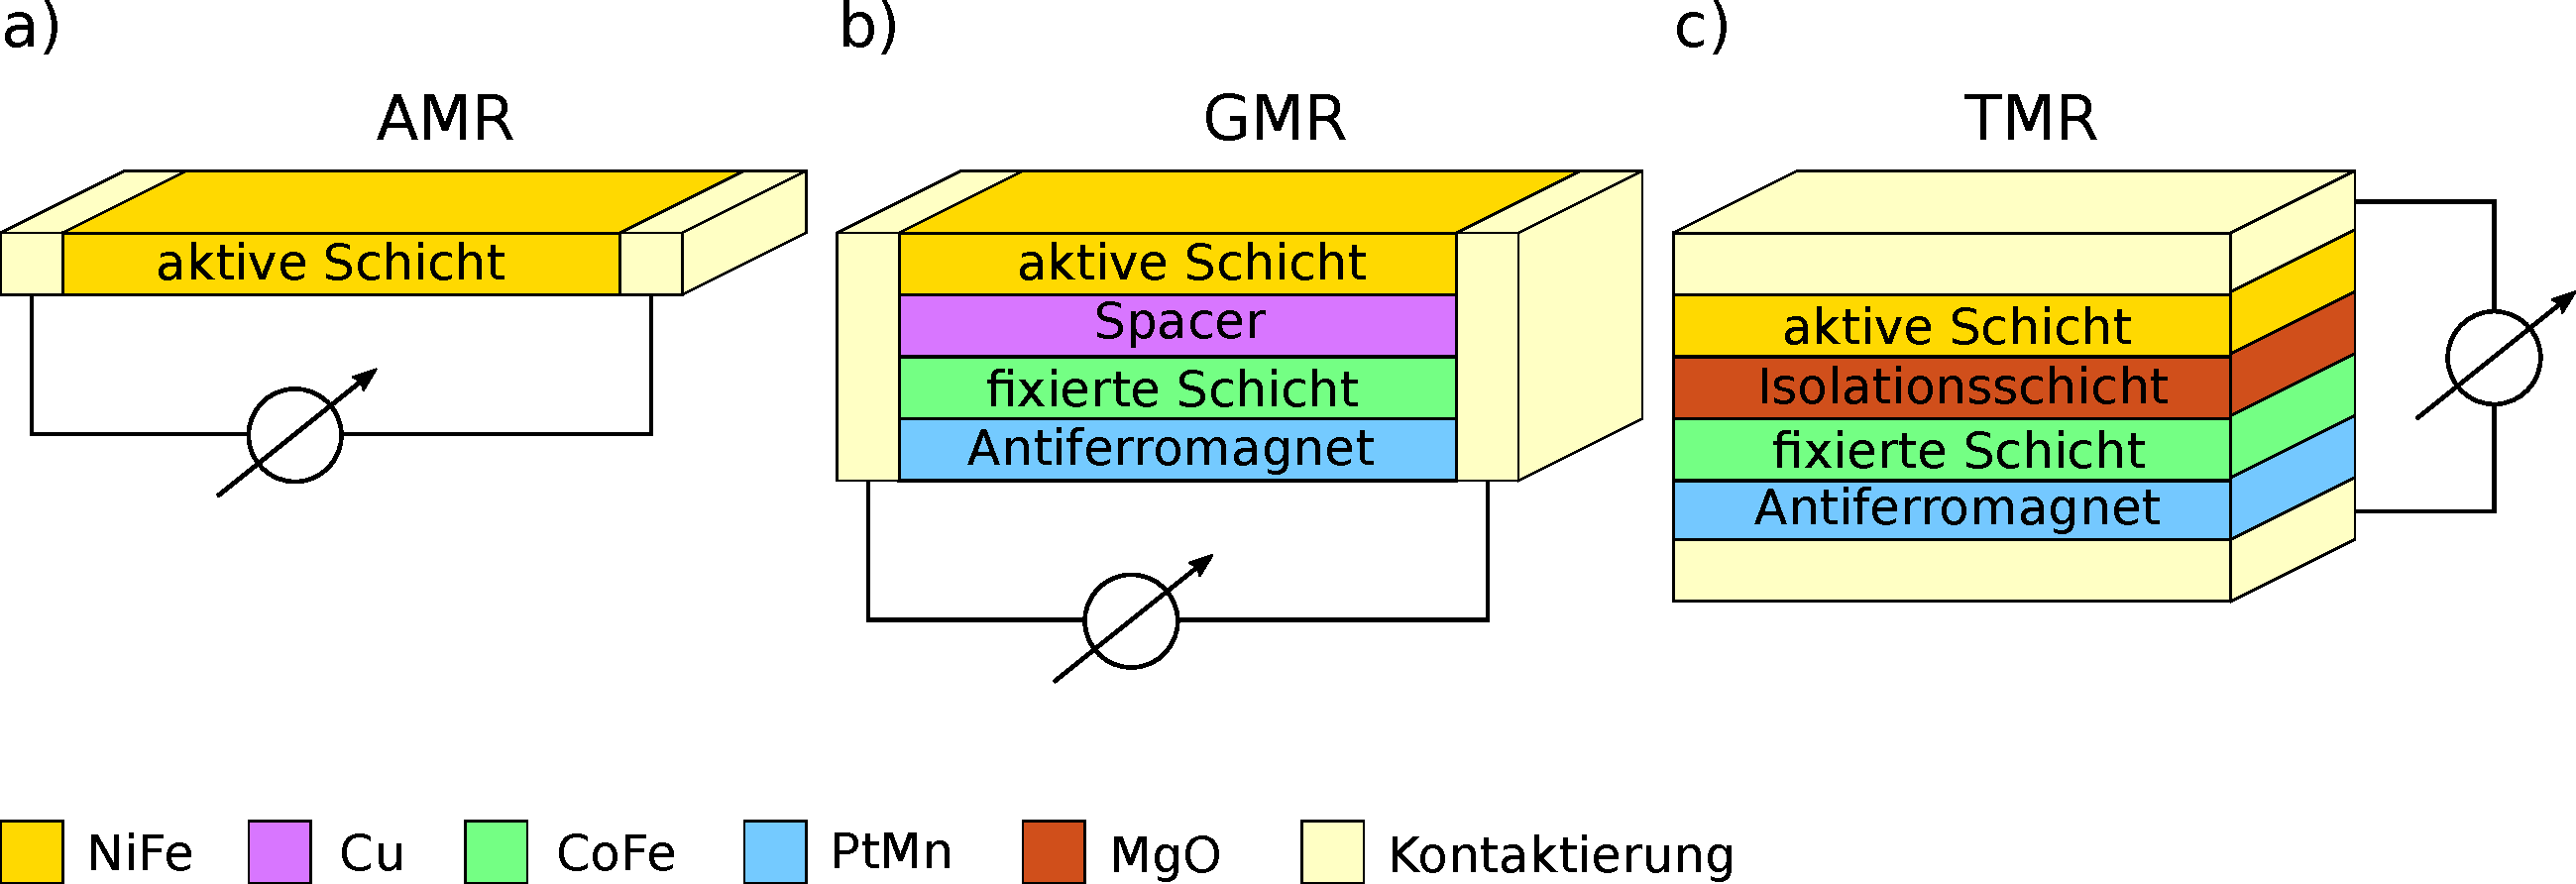
\includegraphics[width=\linewidth]{chapters/images/2-Grundlagen/MR_Schichtmodelle}
	\caption[Schichtmodelle dreier magnetoresistive Effekte]{Schichtmodelle dreier magnetoresistive Effekte. a) 
		\gls{gl:amr}, schwache Widerstandsänderung. b) \gls{gl:gmr} stärkere Widerstandsänderung. c) \gls{gl:tmr} stärkste 
		Widerstandsänderung. Grafik entnommen aus \cite{Lemme2016}.}
	\label{fig:mrschichtmodelle}
\end{figure}


\clearpage


\paragraph{AMR-Effekt}\label{par:AMR}$~$\\


In der Mitte des 19. Jahrhunderts entdeckte der britische Physiker William Thomson den anisotropen magnetoresistiven Effekt (AMR). Der \gls{gl:amr} basiert auf einer von Strom- und Magnetisierungsrichtung abhängigen Streuung von Elektronen in einer einzelnen aktiven Schicht, Teil a) der \autoref{fig:mrschichtmodelle}. Diese Schicht besteht in der Praxis oftmals aus einer Nickel-Eisen-Legierung. Die typische Variation der relativen Widerstandsänderung $\Delta R/R$ liegt im Bereich von $2\%$ bis $3\%$ \cite{Tille2020}. Für eine eindeutig Winkelmessung werden zwei Wheatstone'sche Brücken aus dem Schichtmaterial aufgebaut. Die Stromdurchflussrichtung ist horizontal. Bedingt durch den \gls{gl:amr} ist eine Periodizität von $\SI{180}{\degree}$ abgedeckt \cite{Lemme2016}\cite{Tille2020}. Ein mittels \gls{gl:amr} entwickelter Sensor für die Drehwinkelerfassung, besitzt daher zwei um $\SI{45}{\degree}$ verdrehte Wheatstone-Brücken. Durch die schwache Widerstandsänderung des Materials ist eine nachgeschaltete Verstärkerschaltung notwendig \cite{NXPSemiconductors2014}.


\paragraph{GMR-Effekt}\label{par:GMR}$~$\\


Der riesiger magnetoresistive Effekt, engl. \gls{ac:gmr},  ist 1988 von Grünberg und Fert entdeckt worden. Beide erhielten dafür 2007 den Nobelpreis für Physik, da unter Ausnutzung des \gls{gl:gmr}s sich die Speicherkapazität von Computerfestplatten stark erhöhen ließ \cite{Lemme2016}. Das Minimalprinzip für einen solchen Sensor bildet sich aus zwei magnetischen Dünnschichten, die durch eine nicht magnetische Schicht (z.B. Kupfer) voneinander getrennt sind. Dabei folgt die Magnetisierung der aktiven Schicht (z.B. Nickel-Eisen) einem von außen angelegten Magnetfeld, während die Magnetisierung der zweiten Schicht (z.B. Kobalt-Eisen) durch eine darunter liegende antiferromagnetische Schicht (z.B. Platin-Mangan) fixiert ist. Die Stromdurchflussrichtung bleibt wie beim AMR horizontal \cite{Lemme2016}\cite{Tille2020}. Die relativen Widerstandsänderung $\Delta R/R$ ist abhängig von der relativen Ausrichtung der Magnetisierungen in beiden magnetischen Schichten und liegt für einfache Schichtsystem, wie in Teil b) der \autoref{fig:mrschichtmodelle} gezeigt, bei etwa $\SI{10}{\percent}$. Die Herstellung eines GMR-Sensors ist deutlich aufwendiger, als es beim \gls{gl:amr} der Fall ist. So können aber in Multilagen mit vielfacher Wiederholung der magnetischen Schichten bis zu
$\SI{80}{\percent}$ $\Delta R/R$ erreicht werden \cite{Tille2020}. Mit der GMR Technologie aufgebaute Drehwinkelsensoren haben eine Periodizität von 360° und besitzen zwei um $\SI{90}{\degree}$ verdrehte Wheatstone-Brücken und ebenfalls nachgeschaltete Verstärkereinheiten \cite{infineon2018}.


\paragraph{TMR-Effekt}\label{par:TMR}$~$\\


Im Jahr 1975 ist der tunnel-magnetoresistive Effekt (TMR) durch M. Jullière entdeckt worden. Im einfachsten Fall, wie Teil c) \autoref{fig:mrschichtmodelle} zeigt, tritt der Effekt bei Schichtsystemen auf, die durch eine isolierende Schicht (z.B. Magnesiumoxid) getrennt sind \cite{Lemme2016}. Die Stromdurchflussrichtung ist im Gegensatz zum AMR und GMR vertikal zu den Schichten. Die relativen Widerstandsänderung $\Delta R/R$ erfolgt in Abhängigkeit zur relativen Ausrichtung der Magnetisierungen beider magnetischen Schichten, die an der Isolationsschicht angrenzen.
\newline
Wie beim GMR folgt die aktive Schicht einem äußeren Magnetfeld, ebenso ist die zweite Schicht durch eine antiferromagnetische Schicht fixiert  \cite{Tille2020}. Der zugrunde liegende Effekt ist aber physikalisch ein gänzlich anderer. Hier ``tunnelt'' der Stromfluss durch die Isolationsschicht. Das ist ein quantenmechanischer Effekt und kann mit Ansätzen der ``normalen'' Physik nicht mehr erklärt werden. Zurückzuführen ist der Effekt auf die Spin-Polarisation der einzelnen Elektroden eines magnetischen Tunnel-Kontaktes \cite{Tille2020}.
\newline
In praktischen Ausführungen bei Raumtemperatur liegen heute relative Widerstandsänderungen $\Delta R/R$ im Bereich von $\SI{30}{\percent}$ bis zu $\SI{200}{\percent}$ und sind somit deutlich höher als beim GMR \cite{Tille2020}. Unter Laborbedingungen konnten bei sehr tiefen Temperaturen mittlerweile Widerstandsänderungen bis zu $\SI{1000}{\percent}$ erreicht werden \cite{Lemme2016}.
\newline
Praxistaugliche Ausführungen von TMR-Sensoren stehen erst seit einigen Jahren zur Verfügung. Die Herstellung eines Sensors erfordert einen enormen apparativen Aufwand und Produktionsanlagen mit entsprechenden Fertigkeiten mussten erst entwickelt werden. Der Aufwand ist mit Vorteilen gegenüber dem AMR- und GMR-Sensor entlohnt worden.
Somit besitzt ein TMR-Sensorelement einen viel höheren Widerstand bei gleicher Abmessung. AMR/ GMR Technologien müssen im Vergleich flächenhungrige Strukturen realisieren. Aufgrund der vergleichsweise kleinen Flächen und einer äußerst geringeren Stromaufnahme ist ein engmaschiger Aufbau von Array-Strukturen möglich \cite{Lemme2016}. TMR-Flächen sind typischer Weise $< \SI{2}{\micro\metre}$ im  Radius. Die hohe Widerstandsänderung generiert entsprechend hohe Signalamplituden in der Magnetfelderfassung, daher kann eine nachgeschaltete Verstärkung entfallen. Es ist eine Periodizität von $\SI{360}{\degree}$ abgedeckt. Ein TMR-Sensor für die Drehwinkelerfassung besteht aus zwei um $\SI{90}{\degree}$ verdrehte Wheatstone-Brücken \cite{TDK2016}.


\clearpage

\paragraph{Wheatstone-Brücke}\label{par:wheatstone-bruecke}$~$\\


Ein einzelnes TMR-Element bzw. Widerstand kann bereits als eigenständiger magnetischer Sensor betrachtet werden. Allerdings können Temperatureinflüsse den Widerstand mitunter variieren lassen. Um dem Temperatureinfluss entgegenzuwirken, werden daher \gls{gl:wheatstonebruecken} genutzt. Die einzelnen Widerstände der Brücke sind dabei so angeordnet, dass sie einen gemeinsamen Temperaturkoeffizienten besitzen und entsprechend miteinander gleichmäßig schwanken \cite{Tille2020}. Über die Differenzmessung an den Brückenmittelabgriffen wird somit der Temperatureinfluss weitestgehend unterdrückt \cite{TDK2016}\cite{Tille2020}. \autoref{fig:tmrdrehwinkelapplikation} zeigt den schematischen Brückenaufbau für einen TMR-Sensor. Bei gleichförmiger Rotation eines Anregungsmagnetfeld wird durch die $\SI{90}{\degree}$-Verdrehung beider Brücken zueinander erreicht, dass die benötigte Cosinus- und Sinus-Funktion, mit entsprechender Phasenverschiebung um $\SI{90}{\degree}$, für den Anwendungsfall in \autoref{sec:kreisdarstellung-anwendung} ausgeben werden \cite{TDK2016}. 


\vspace{5mm}
\begin{figure}[tbph]
	\centering
	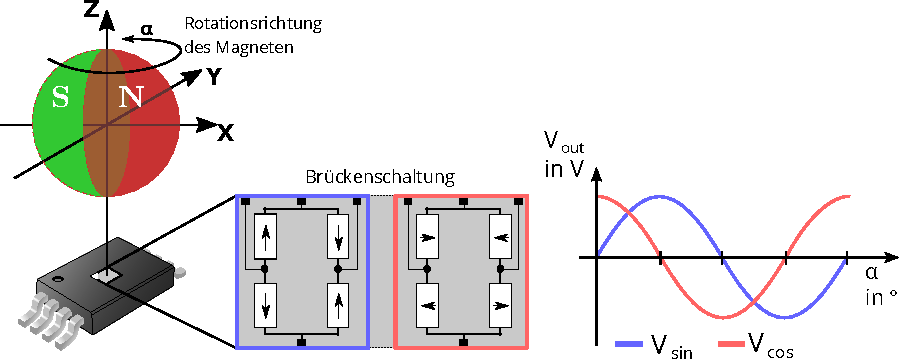
\includegraphics[width=\linewidth]{chapters/images/2-Grundlagen/TMR_Drehwinkelapplikation}
	\caption[TMR Drehwinkelapplikation]{TMR Drehwinkelapplikation. Schematisch gezeigt für eine volle Rotation des 
		Gebermagneten um $\SI{360}{\degree}$. Zu sehen sind die um $\SI{90}{\degree}$ verdrehten Wheatstone-Brücken des 
		Sensors. Die Brücken bilden, bei rotierendem Gebermagnetfeld, eine Sinus- und Cosinus-Funktion nach. Die Pfeile in 
		den einzelnen Widerständen weisen auf ihre magnetische Ausrichtung hin. Grafik entnommen und bearbeitet aus 
		\cite{Schuethe2020a}.}
	\label{fig:tmrdrehwinkelapplikation}
\end{figure}
